\documentclass[a4paper,masters,10pt]{york-thesis}
\usepackage{amsmath}
\usepackage{amsfonts}
\usepackage{amssymb}
\usepackage{stmaryrd}
\usepackage{multicol}
\usepackage{listings}
\usepackage{lscape}
\usepackage{enumerate}
%\usepackage{floatflt, wrapfig, epsfig}
%\usepackage{color}
\usepackage{xspace}
\usepackage{theorem}
%\usepackage{makeidx}
%\usepackage{ifthen}
%\usepackage{fancyhdr}
\usepackage[pdftex]{graphicx}                  
%\usepackage{multirow}
\usepackage{verbatim} 
%\usepackage{rotating}
%\FrenchItemizeSpacingfalse
\bibliographystyle{apalike}
\usepackage[latin1]{inputenc}
\usepackage[T1]{fontenc}
\usepackage[english]{babel}
\usepackage{pgf}
\usepackage{color}
\usepackage{xcolor}
\usepackage{xxcolor}
\usepackage{tikz}
\usepackage{pgflibraryarrows}
\usepackage{multido}
\usepackage{amsmath}
\usepackage{multirow}
    
\selectlanguage{english}

\pdfinfo{
	/Title (XLPython)
	/Creator (S�bastien Lapedra)
	/Producer (pdfLaTeX)
	/Author (S�bastien Lapedra)
	/Subject (Excel Python)
}


\newcommand{\xlp}{{\sc XLPython }}

\newcommand{\probaspace}{$(\Omega,\filtr,\proba)$}


\newcommand{\onelevytriplet}{$(b,\sigma,\upsilon)$}


\newcommand{\intR}{\ensuremath{\int_{\Rnb}}}


\newcommand{\mlinea}{
\begin{tikzpicture}
\pgfsetlinewidth{0.15ex}
\draw[-,scale=1] (13,0) -- (18,0);
\end{tikzpicture}}

\newcommand{\mline}{
\begin{tikzpicture}
\pgfsetlinewidth{0.15ex}
\draw[-,scale=1] (0,0) -- (15.3,0);
\end{tikzpicture}}

\newcommand{\mlineb}{
\begin{tikzpicture}
\pgfsetlinewidth{0.15ex}
\draw[-,scale=1] (0,0) -- (5,0);
\end{tikzpicture}}

\definecolor{mred}{rgb}{0.30,0.00,0.00}
\definecolor{mblue}{rgb}{0.10,0.20,0.50}




\newenvironment{xlpfunc}[1]
{
\

\textcolor{mblue}{\textsc{\textbf{#1}}}

\vspace{2mm}

\hfill\begin{minipage}[t]{.90\linewidth}
}
{\end{minipage}
\vspace{3mm}}

\newenvironment{xlpfunctitle}[1]
{
\

\mlinea\hfill\textcolor{mblue}{\textsc{\textbf{#1}}}\hfill\mlineb

\vspace{2mm}
\begin{minipage}[t]{1.0\linewidth}
}
{
\mline
\end{minipage}
\vspace{3mm}}



\begin{document}

\nocite{*}


\title{Interest Rate: Derivatives Pricing and Models}
\author{Lapedra S�bastien}
\begin{titlepage}
		
\begin{center}
	\end{center}
	\vfill
	\begin{center}
   	
   	 
  	\begin{center}
			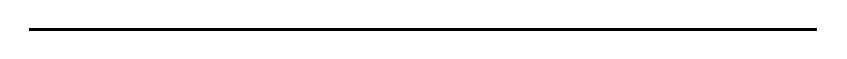
\begin{tikzpicture}
				\pgfsetlinewidth{0.3ex}
				\draw[-,scale=1] (0,0) -- (10,0);
			\end{tikzpicture}
		\end{center}
		
		\ 
		
		\
		
    {\huge XLPython 1.0.0}

    \

     {\huge Excel Python}
		
		\
		
		\
		  
		 {\large\scshape Lapedra S�bastien}
		 \
		 
		\begin{center}
			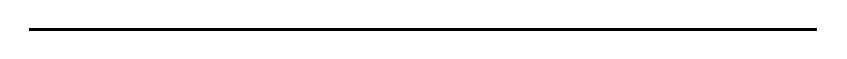
\begin{tikzpicture} 
				\pgfsetlinewidth{0.3ex}
				\draw[-,scale=1] (0,0) -- (10,0);
			\end{tikzpicture}
		\end{center}
		
     
	\end{center}
	\vfill	
	\vfill
	\vfill
%	\begin{center}
%			\begin{tikzpicture}
%				\pgfsetlinewidth{0.3ex}
%				\draw[-,scale=1] (0,0) -- (15,0);
%			\end{tikzpicture}
%		\end{center}
%	\begin{center}
%\begin{tabular}{p{8cm}p{8cm}}
%	 \includegraphics[width=8cm]{images/logofideuram.jpg} \hfill& \hfill 
%	 \includegraphics[width=2cm]{images/logoeuria.jpg}\\
%	\end{tabular}
%	\end{center}

\end{titlepage}


\tableofcontents
%\addcontentsline{toc}{chapter}{Table des matiu�res}
%\listoftables
%\addcontentsline{toc}{chapter}{Liste des tableaux}
%\listoffigures
%\addcontentsline{toc}{chapter}{Table des figures}

\chapter{Introduction}

This document is geared towards people who a have an intermediate level in python programming and Excel.

\

\xlp is an Excel add-in who implement the {\it Object Handler Concept} in Python. By {\it Object Handler Concept}, meaning the way of using object instance directly in Excel.

\xlp is composed of a set of excel functions directly available (after having installed the add-in) on Excel.

\

This document is divided in three part: 
\begin{itemize}
\item how to install and getting started with \xlp
\item architecture of \xlp
\item tutorials.
\end{itemize}









\chapter{Getting started}

\section{Installation}

Before installing \xlp you need to install python. \xlp has been tested with version 2.5 of python. We suggest you to install this version.

\

Once python is installed, go to the directory {\it I:/Bjb\_App/Arena/Quants/xlpython}. Open excel, menu Tools -> Addins, install xlpython.xll (say yes to copy on your computer). 

\

Open the file xlp-example.xll to check the installation. 

\section{\xlp Concept}


\xlp is an Excel add-in. Which provides some new functions available into the function wizard. 

\xlp implements the  {\it Object Handler Concept} using the functionalitiy of Python. Is to say that you will create python object instances directly into a worksheet, instances can in turn be used for future calculations.

\

An example is always better.

\

Imagine that you have a data set which represents a rate term structure:

\begin{center}
\begin{tabular}{c|c}
\bf{Maturity (year fraction)} & rate \\
\hline\\
1.00 & 3.60\% \\
2.00 & 4.60\% \\
3.00 & 5.60\% \\
4.00 & 6.60\% 
\end{tabular}
\end{center}

Your aim is to interpolate the rate term structure linearly for a set of times ${1.5, 2.5, 3.5}$.

\

One solution will be to use a interpolation function, named {\it linear\_interpolate}, that will take 3 argument vectors: the rates, the times and the time where you want to interpolate.  

\begin{center}
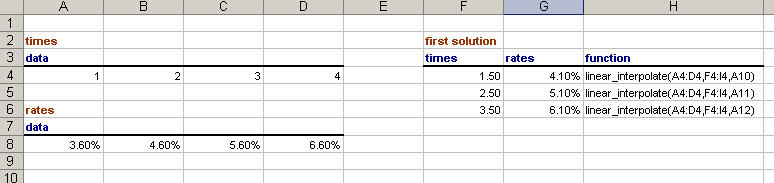
\includegraphics[width=16cm]{images/intex1.jpg}
\end{center}

This solution is simple but you can immediately see that this has a lot of drawbacks:

\begin{itemize}
\item You have to specify the input data every time you want to interpolate. That increase the possibility to make mistakes.
\item For each interpolation, you need to perform the same calculation on the same data even if they do not change, that cause a performance decrease. 
\end{itemize}

\

Another solution is to use objects and keep a record of theses objects into Excel.

\begin{center}
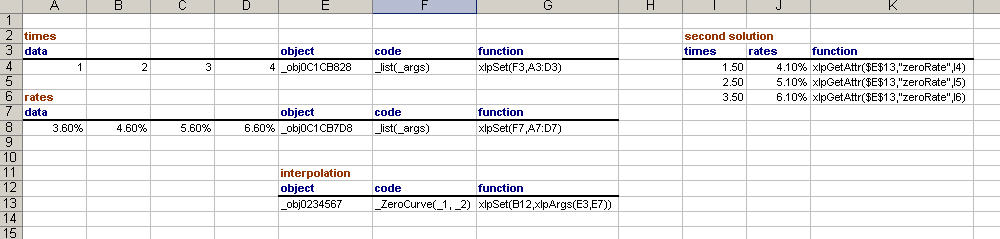
\includegraphics[width=16cm]{images/intex2.jpg}
\end{center}

As seen on the figure above, first we create objects which represents times and rates. With this two objects we compose a {\it ZeroCurve} object. Then we use this object to obtain the value of the interpolation.

This solution is more complex than the first use but it is more efficient.



\chapter{Architecture of \xlp}

\xlp is composed of a set of functions. These functions are directly available in Excel, grouped into a category called \xlp.


\

Conceptually functions can be divided into 6 categories:

\begin{itemize}
\item python execution functions,
\item object management functions,
\item output functions,
\item tool functions.
\item information functions,
\end{itemize} 

In the next sections we will investigate the usage of each function.

\begin{figure}
\begin{minipage}[t]{.55\linewidth}
\begin{tabular}{ll}
\multicolumn{2}{l}{\textbf{\textcolor{mred}{execution functions}}} \\
\textbf{\textcolor{mblue}{name}} & \textbf{\textcolor{mblue}{arguments}}  \\
\hline\\
{\sl \bf xlpSet} &  scalar, args, values, index, id, trigger\\
{\sl \bf xlpGet} & scalar, args, transpose, trigger \\
{\sl \bf xlpCommandGet} & scalar, args, output, transpose\\
{\sl \bf xlpApply} &  scalar, args, id, trigger\\
{\sl \bf xlpGetApply} & scalar, args, transpose, trigger \\
{\sl \bf xlpCommandGetApply} & scalar, args, output, transpose\\
{\sl \bf xlpAttr} &  scalar, args, values, index, id, trigger\\
{\sl \bf xlpGetAttr} & scalar, args, transpose, trigger \\
{\sl \bf xlpCommandGetAttr} & scalar, args, output, transpose\\
{\sl \bf xlpExec} & code, args, ids, transpose, trigger \\
{\sl \bf xlpExecFile} & filename, args, ids, transpose, trigger \\
{\sl \bf xlpImport} & scalar, id, trigger \\
{\sl \bf xlpFromImport} & scalar, trigger \\
{\sl \bf xlpInsertPaths} & paths, trigger \\
\end{tabular}
\end{minipage}\hfill
\begin{minipage}[t]{.30\linewidth}
\begin{tabular}{ll}
\multicolumn{2}{l}{\textbf{\textcolor{mred}{output functions}}} \\
\textbf{\textcolor{mblue}{name}} & \textbf{\textcolor{mblue}{arguments}}  \\
\hline\\
{\sl \bf xlpFullIO} &  trigger\\
{\sl \bf xlpIO} & lines, trigger \\
& \\
& \\
& \\
& \\
& \\
& \\
& \\
& \\
& \\
& \\
& \\
& \\
& 
\end{tabular}
\end{minipage}
\vspace{10mm}

\begin{minipage}[t]{.55\linewidth}
\begin{tabular}{ll}
\multicolumn{2}{l}{\textbf{\textcolor{mred}{object management functions}}} \\
\textbf{\textcolor{mblue}{name}} & \textbf{\textcolor{mblue}{arguments}}  \\
\hline\\
{\sl \bf xlpType} &  scalar, trigger\\
{\sl \bf xlpListAllObjects} & transpose, trigger \\
{\sl \bf xlpDeleteAllObjects} & trigger \\
{\sl \bf xlpDeleteObject} & scalar, trigger \\
{\sl \bf xlpListAllAttr} & scalar, transpose, trigger \\
{\sl \bf xlpListAttrInfos} & scalar, attr, transpose, trigger
\end{tabular}
\end{minipage}\hfill
\begin{minipage}[t]{.30\linewidth}
\begin{tabular}{ll}
\multicolumn{2}{l}{\textbf{\textcolor{mred}{information functions}}} \\
\textbf{\textcolor{mblue}{name}} & \textbf{\textcolor{mblue}{arguments}}  \\
\hline\\
{\sl \bf xlpVersion} & trigger \\
{\sl \bf xlpAuthor} &  trigger \\
{\sl \bf xlpContributors} & trigger \\
{\sl \bf xlpPythonPath} & trigger \\
{\sl \bf xlpPythonVersion} & trigger \\
{\sl \bf xlpSysPaths} & trigger 
\end{tabular}
\end{minipage}

\vspace{10mm}
 
\begin{minipage}[t]{.80\linewidth}
\begin{tabular}{ll}
\multicolumn{2}{l}{\textbf{\textcolor{mred}{tool functions}}} \\
\textbf{\textcolor{mblue}{name}} & \textbf{\textcolor{mblue}{arguments}}  \\
\hline\\
{\sl \bf xlpArgs} &  args01, args02, args03, args04, args05, transpose, trigger \\
{\sl \bf xlpBigArgs} &  args01, args02, ... argsXX ... args18, transpose, trigger \\
{\sl \bf xlpTrigger} &  trigger01, trigger02, trigger03, trigger04, trigger05\\
{\sl \bf xlpBigTrigger} &  trigger01, trigger02, ... triggerXX ... trigger20\\
{\sl \bf xlpTranspose} & scalar, trigger \\
{\sl \bf xlpT} & scalar, trigger \\
{\sl \bf xlpAdjustShape} & scalars, rows, columns, transpose, trigger \\
{\sl \bf xlpLoadFile} & file, id, trigger \\
{\sl \bf xlpVolatile} & trigger \\
{\sl \bf xlpReduce} & arguments, transpose, trigger \\
{\sl \bf xlpR} & arguments, transpose, trigger \\
{\sl \bf xlpPretty} & arguments, transpose, trigger \\
{\sl \bf xlpP} & arguments, transpose, trigger \\
{\sl \bf xlpTime} & trigger \\
\end{tabular}
\end{minipage}
\caption{\xlp functions}
\end{figure}

\section{Managing object and python into Excel}

An Excel cell can handle different kind of data: 

\begin{itemize}
\item real numbers 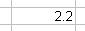
\includegraphics[width=1.4cm]{images/real.jpg}
\item character strings 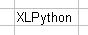
\includegraphics[width=1.4cm]{images/string.jpg}
\item booleans 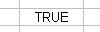
\includegraphics[width=1.4cm]{images/bool.jpg}
\item others irrelevant type.
\end{itemize}

\xlp will directly map thes types to equivalent python types except for the character string. We need a way to differentiate character string from python code. For that purpose, \xlp impose a limitation on string types. Every string that begins by the character {\bf \_} will be interpret as python code.

\

That means that:

\begin{itemize}
\item 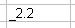
\includegraphics[width=1.4cm]{images/preal.jpg} will be interpreted as a real number,
\item 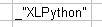
\includegraphics[width=1.4cm]{images/pstring.jpg} will be interpreted as a string,
\item 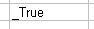
\includegraphics[width=1.4cm]{images/pbool.jpg} will be interpreted as a boolean.
\end{itemize}

This solution brings flexibility. For example: 

\begin{itemize}
\item 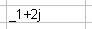
\includegraphics[width=1.4cm]{images/complex.jpg} will be interpreted as a complex number,
\item 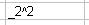
\includegraphics[width=1.4cm]{images/square.jpg} will be interpreted as a real of value $4.0$.
\end{itemize}

\section{Output cell selection}

The result of each function is a cell matrix (Ctr+Shift+Enter on Excel).

\section{The trigger argument}

In Excel, a function can be declared as {\it volatile}. {\it Volatile} means that the function will be executed when the sheet will be recalculated. That behaviour can lead to troubles. Imagine that you have a long monte-carlo simulation. You cannot accept to compute the simulation every time that you make a modification on your sheet. That is why all the functions of \xlp, except one, are declared as non volatile. However, we need a way to control when a function wil be calculated again. The solution is to add and additionnal argument, called trigger, that will or not refers to another cell. If the trigger refer to another cell, and we modify that cell, Excel will automaticaly calculate again the function. So by controling the value of that cell we control the computation of the functions.


\

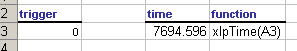
\includegraphics[width=7cm]{images/trigger1.jpg} \hfill 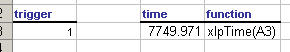
\includegraphics[width=7cm]{images/trigger2.jpg}

\

All the \xlp functions have a trigger argument.

\

A FALSE value trigger will invalidate the function.

\

We mentioned above that one function is declared as volatile. This function is called {\sl xlpVolatile} and its role is to allow to have volatile triggers and so on volatile functions. 

\section{Argument bindings and placeholder definitions}

Excel, like all spreadsheet application, is powerfull to generic calculation with cells. In order to bring that functionality to python, an argument binding methododlogy is implemented in \xlp. That method consists in creating local variables directly available into a python script.  

\

These local variables will be accessible in python. They will begin by "\_". For example the variable "\_size" will be filled with the size of arguments list. See the next section for more details.

\section{Argument convention}

The same argument passing convention has been used for all the functions.

\begin{itemize}
\item \textsl{scalar} is a real number, a boolean or a character string (including python character strings and scripts).
\item \textsl{args} is a selection of scalars with specific binding to a python list named "\_args". Each element of the list is directly accessible in python with the placeholder syntax "\_1", "\_2" ... "\_n" where n represents the index of the element in the list. "\_size" will be the global size of the selection, "\_rows" will be the number of rows of the selection and "\_cols" will be the number of columns of the selection.
\item \textsl{values} is a selection of scalars with specific binding to a python list "\_values". \textcolor{mred}{if no \textsl{args} argument is defined} "\_size" will be the global size of the selection, "\_rows" will be the number of rows of the selection and "\_cols" will be the number of columns of the selection. 
\item \textsl{index} is a selection of scalars with specific binding to a python list "\_index". 
\item \textsl{id} is a character string which give a name to a python object. If this argument is empty an automatic name will be given. The name can contain any alphnumeric character plus the "\_" character except in first position.
\item \textsl{transpose} is a boolean used to transpose the ouput cell. The default value is FALSE and correspond to writing datas from the top to the bottom output cell selection line by line.  
\item \textsl{trigger} is a trigger reference. 
\end{itemize}


\section{Python execution functions}

\subsection{xlpSet}

\begin{xlpfunctitle}{xlpSet}

\begin{xlpfunc}{Parameters}
\begin{tabular}{p{3.5cm}cl}
\textbf{scalar}& : & scalar code \\
\textbf{args}& : & list or arguments \\
\textbf{values}& : & list of values \\
\textbf{index}& : & list of index  \\
\textbf{id}& : & object id \\
\textbf{trigger}& : & trigger \\
\end{tabular}

\vspace{2mm}

index and values must have the same size if index is passed.
\end{xlpfunc}


\begin{xlpfunc}{Returns}
A character string representing the python object created
\end{xlpfunc}

\begin{xlpfunc}{Description}
Execute python code and store the result into a python object. It is the core function of \xlp. 

\

The values and index argument are used to fill container in a generic way.

\

The function creates an object with the scalar and args information. If the argument values is not empty and the object implement the \_\_setitem\_\_ method, the function will try to fill the object with the data contained in values. 

If the index argument is not empty, the elements of index argument will be used as the index parameter of the \_\_setitem\_\_ method. Otherwise, $\{1, ..., n\}$ will be used.

\

\textbf{Argument bindings} : \_args, \_size, \_rows, \_cols, \_1 ... \_n

\

If the scalar argument corresponds to a python code that does not return an object, xlpSet will return an object of NoneType. 

\

values and index arguments are automatically reduce (see xlpReduce for more details).

\

Two local function are available for creating objects:
\begin{itemize}
\item \_listlist(rows, columns, args): that create a list of list of dimenstions (rows, columns) filling the data with arguments (cf. xlp-example.xls).
\item \_extstr(rows, columns, args): that create a string from a cell matrix putting tabular character when a column jump appears and new line character when a row jump appears (cf. xlp-example.xls).
\end{itemize}

\end{xlpfunc}

\end{xlpfunctitle}

\subsection{xlpGet}

\begin{xlpfunctitle}{xlpGet}

\begin{xlpfunc}{Parameters}
\begin{tabular}{p{3.5cm}cl}
\textbf{scalar}& : & scalar code \\
\textbf{args}& : & list or arguments \\
\textbf{transpose}& : & transpose   \\
\textbf{trigger}& : & trigger \\
\end{tabular}

\vspace{2mm}

\end{xlpfunc}


\begin{xlpfunc}{Returns}
A cell matrix.
\end{xlpfunc}

\begin{xlpfunc}{Description}
Get data from python and display it in Excel. This method is generic and can handled only types:
\begin{itemize}
\item float
\item str
\item bool
\item NoneType
\item complex
\item other types that implement {\sl \_\_getitem\_\_} method and/or the {\sl size} method. 
\end{itemize}

The {\sl size} method return a tuple with the dimensions of the object to show. Obviously \xlp cannot handle more than two dimensions. That means that a matrix object will return a tuple of size 2 and a vector a tuple of size 1.

\

xlpGet as a specific behaviour with character string. \xlp interprets the tabular caharacter to jump to a new column and the new line character to jump to a new row. That means that this sentence "Hello <tabular> this	<tabular> is a <newline> test <tabular>	message	<newline> The name <tabular> of <tabular>	XLPython <newline> is	<tabular> XLPython" will be show as: 

\

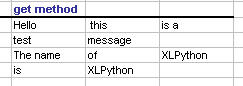
\includegraphics[width=6cm]{images/extstr2.jpg}


\

\textbf{Argument bindings} : \_args, \_size, \_rows, \_cols, \_1 ... \_n



\end{xlpfunc}
\end{xlpfunctitle}



\subsection{xlpPrettyGet}

\begin{xlpfunctitle}{xlpCommandGet}

\begin{xlpfunc}{Parameters}
\begin{tabular}{p{3.5cm}cl}
\textbf{scalar}& : & scalar code \\
\textbf{args}& : & list or arguments \\
\textbf{output}& : & output cell matrix\\
\textbf{transpose}& : & transpose   \\
\end{tabular}

\vspace{2mm}

\end{xlpfunc}


\begin{xlpfunc}{Returns}
A cell matrix.
\end{xlpfunc}

\begin{xlpfunc}{Description}
Same as xlpGet but the result is written on the ouput cell matrix. This function can only be called from VBA. "success" is returned in case of success or "more" if the output cell matris is not big enough to contain all the result.
\end{xlpfunc}
\end{xlpfunctitle}


\subsection{xlpApply}

\begin{xlpfunctitle}{xlpApply}

\begin{xlpfunc}{Parameters}
\begin{tabular}{p{3.5cm}cl}
\textbf{scalar}& : & scalar code \\
\textbf{args}& : & list or arguments \\
\textbf{id}& : & object id   \\
\textbf{trigger}& : & trigger \\
\end{tabular}

\vspace{2mm}

\end{xlpfunc}


\begin{xlpfunc}{Returns}
A character string representing the python object created
\end{xlpfunc}

\begin{xlpfunc}{Description}
Apply a callable object with args arguments.

\

\textbf{Argument bindings} : \_args, \_size, \_rows, \_cols, \_1 ... \_n

\end{xlpfunc}
\end{xlpfunctitle}


\subsection{xlpGetApply}

\begin{xlpfunctitle}{xlpGetApply}

\begin{xlpfunc}{Parameters}
\begin{tabular}{p{3.5cm}cl}
\textbf{scalar}& : & scalar code \\
\textbf{args}& : & list or arguments \\
\textbf{transpose}& : & transpose \\
\textbf{trigger}& : & trigger \\
\end{tabular}

\vspace{2mm}

\end{xlpfunc}


\begin{xlpfunc}{Returns}
A cell matrix.
\end{xlpfunc}

\begin{xlpfunc}{Description}
Apply a callable object with args arguments and return the result.

\

\textbf{Argument bindings} : \_args, \_size, \_rows, \_cols, \_1 ... \_n

\end{xlpfunc}
\end{xlpfunctitle}

\subsection{xlpCommandGetApply}

\begin{xlpfunctitle}{xlpPrettyGetApply}

\begin{xlpfunc}{Parameters}
\begin{tabular}{p{3.5cm}cl}
\textbf{scalar}& : & scalar code \\
\textbf{args}& : & list or arguments \\
\textbf{output}& : & output cell matrix\\
\textbf{transpose}& : & transpose
\end{tabular}

\vspace{2mm}

\end{xlpfunc}


\begin{xlpfunc}{Returns}
A cell matrix.
\end{xlpfunc}

\begin{xlpfunc}{Description}
The version of xlpCommandGet fo xlpGetApply.

\

\textbf{Argument bindings} : \_args, \_size, \_rows, \_cols, \_1 ... \_n

\end{xlpfunc}
\end{xlpfunctitle}












\subsection{xlpAttr}

\begin{xlpfunctitle}{xlpAttr}

\begin{xlpfunc}{Parameters}
\begin{tabular}{p{3.5cm}cl}
\textbf{scalar}& : & scalar code \\
\textbf{attr}& : & attribute \\
\textbf{args}& : & list or arguments \\
\textbf{id}& : & object id   \\
\textbf{trigger}& : & trigger \\
\end{tabular}

\vspace{2mm}

\end{xlpfunc}


\begin{xlpfunc}{Returns}
A character string representing the python object created
\end{xlpfunc}

\begin{xlpfunc}{Description}
Apply an attribute object with args arguments if callable or get an attribute object.

\

\textbf{Argument bindings} : \_args, \_size, \_rows, \_cols, \_1 ... \_n

\end{xlpfunc}
\end{xlpfunctitle}


\subsection{xlpGetAttr}

\begin{xlpfunctitle}{xlpGetAttr}

\begin{xlpfunc}{Parameters}
\begin{tabular}{p{3.5cm}cl}
\textbf{scalar}& : & scalar code \\
\textbf{args}& : & list or arguments \\
\textbf{transpose}& : & transpose \\
\textbf{trigger}& : & trigger \\
\end{tabular}

\vspace{2mm}

\end{xlpfunc}


\begin{xlpfunc}{Returns}
A cell matrix.
\end{xlpfunc}

\begin{xlpfunc}{Description}
Same as xlpAttr but returning directly the result and not an object.

\

\textbf{Argument bindings} : \_args, \_size, \_rows, \_cols, \_1 ... \_n

\end{xlpfunc}
\end{xlpfunctitle}

\subsection{xlpCommandGetAttr}

\begin{xlpfunctitle}{xlpPrettyGetAttr}

\begin{xlpfunc}{Parameters}
\begin{tabular}{p{3.5cm}cl}
\textbf{scalar}& : & scalar code \\
\textbf{args}& : & list or arguments \\
\textbf{output}& : & output cell matrix\\
\textbf{transpose}& : & transpose \\
\end{tabular}

\vspace{2mm}

\end{xlpfunc}


\begin{xlpfunc}{Returns}
A cell matrix.
\end{xlpfunc}

\begin{xlpfunc}{Description}
The version of xlpCommandGet fo xlpGetAttr

\

\textbf{Argument bindings} : \_args, \_size, \_rows, \_cols, \_1 ... \_n

\end{xlpfunc}
\end{xlpfunctitle}









\subsection{xlpExec}


\begin{xlpfunctitle}{xlpExec}

\begin{xlpfunc}{Parameters}
\begin{tabular}{p{3.5cm}cl}
\textbf{code}& : & script code \\
\textbf{args}& : & list or arguments \\
\textbf{ids}& : & list of ids \\
\textbf{transpose}& : & output transpose \\
\textbf{trigger}& : & trigger \\
\end{tabular}
\end{xlpfunc}


\begin{xlpfunc}{Returns}
A cell matrix of dimension (1, n) where n is the number of created objects  
\end{xlpfunc}

\begin{xlpfunc}{Description}
Execute python script written directly into Excel cells. The returns cell matrix represent the object ids.


\

A special object is available in order to return data. This object is "\_" and has just one method "operator+=". The usage is "\_ += object\_to\_return" in order to allow object to be available in Excel.

If you define any object into your code, you can also declare it as global in order that it will be available for future python call.

\

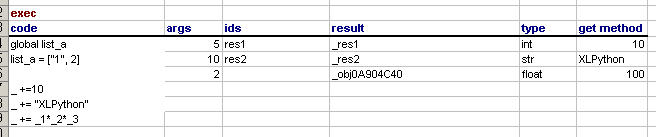
\includegraphics[width=11cm]{images/exec.jpg}

\

\textbf{Argument bindings} : \_args, \_size, \_rows, \_cols, \_1 ... \_n
 
\end{xlpfunc}
\end{xlpfunctitle}



\subsection{xlpExecFile}


\begin{xlpfunctitle}{xlpExecFile}

\begin{xlpfunc}{Parameters}
\begin{tabular}{p{3.5cm}cl}
\textbf{code}& : & script code \\
\textbf{args}& : & list or arguments \\
\textbf{ids}& : & list of ids \\
\textbf{transpose}& : & output transpose \\
\textbf{trigger}& : & trigger \\
\end{tabular}
\end{xlpfunc}


\begin{xlpfunc}{Returns}
A cell matrix of dimension (1, n) where n is the number of created object  
\end{xlpfunc}

\begin{xlpfunc}{Description}
Same as xlpExec but getting the python script from a file.

\

\textbf{Argument bindings} : \_args, \_size, \_rows, \_cols, \_1 ... \_n
 
\end{xlpfunc}
\end{xlpfunctitle}



\subsection{xlpImport}


\begin{xlpfunctitle}{xlpImport}

\begin{xlpfunc}{Parameters}
\begin{tabular}{p{3.5cm}cl}
\textbf{scalar}& : & scalar code\\
\textbf{id}& : & object id \\
\textbf{trigger}& : & trigger \\
\end{tabular}
\end{xlpfunc}


\begin{xlpfunc}{Returns}
A character string representing the object id of the imported module. 
\end{xlpfunc}

\begin{xlpfunc}{Description}
Import a python module with name given by id. If id is missing, the imported module name will be the same as the module name. 
\end{xlpfunc}
\end{xlpfunctitle}


\subsection{xlpFromImport}


\begin{xlpfunctitle}{xlpFromImport}

\begin{xlpfunc}{Parameters}
\begin{tabular}{p{3.5cm}cl}
\textbf{scalar}& : & scalar code\\
\textbf{trigger}& : & trigger \\
\end{tabular}
\end{xlpfunc}


\begin{xlpfunc}{Returns}
"success" in case of no error. 
\end{xlpfunc}

\begin{xlpfunc}{Description}
Same as "from module\_name" import *. 
\end{xlpfunc}
\end{xlpfunctitle}


\subsection{xlpFromImport}


\begin{xlpfunctitle}{xlpInsertPaths}

\begin{xlpfunc}{Parameters}
\begin{tabular}{p{3.5cm}cl}
\textbf{paths}& : & list of paths to include \\
\textbf{trigger}& : & trigger \\
\end{tabular}
\end{xlpfunc}


\begin{xlpfunc}{Returns}
"success" in case of no error.
\end{xlpfunc}

\begin{xlpfunc}{Description}
Insert paths in the python system path (check for duplication).
\end{xlpfunc}
\end{xlpfunctitle}




\section{Object management functions}


\subsection{xlpType}

\begin{xlpfunctitle}{xlpType}

\begin{xlpfunc}{Parameters}
\begin{tabular}{p{3.5cm}cl}
\textbf{scalar}& : & scalar code \\
\textbf{trigger}& : & trigger 
\end{tabular}
\end{xlpfunc}


\begin{xlpfunc}{Returns}
A cell matrix of dimension (1, 1)
\end{xlpfunc}

\begin{xlpfunc}{Description}
Return the type of scalar. 
\end{xlpfunc}
\end{xlpfunctitle}


\subsection{xlpListAllObjects}

\begin{xlpfunctitle}{xlpListAllObjects}

\begin{xlpfunc}{Parameters}
\begin{tabular}{p{3.5cm}cl}
\textbf{transpose}& : & transpose ouput \\
\textbf{trigger}& : & trigger 
\end{tabular}
\end{xlpfunc}

\begin{xlpfunc}{Returns}
A cell matrix of dimension (2, n)
\end{xlpfunc}

\begin{xlpfunc}{Description}
Return all the python objects. The first column is the object name, the second column is the type of the object 

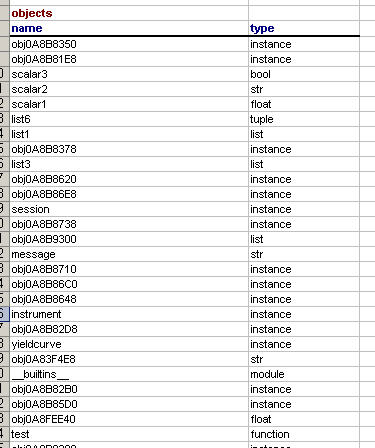
\includegraphics[width=8cm]{images/objects.jpg}
\end{xlpfunc}
\end{xlpfunctitle}


\subsection{xlpDeleteAllObjects}

\begin{xlpfunctitle}{xlpDeleteAllObjects}

\begin{xlpfunc}{Parameters}
\begin{tabular}{p{3.5cm}cl}
\textbf{trigger}& : & trigger 
\end{tabular}
\end{xlpfunc}


\begin{xlpfunc}{Returns}
Character string equal to "success" in case of no error.
\end{xlpfunc}

\begin{xlpfunc}{Description}
Delete all objects.
\end{xlpfunc}
\end{xlpfunctitle}

\subsection{xlpDeleteObject}

\begin{xlpfunctitle}{xlpDeleteObject}

\begin{xlpfunc}{Parameters}
\begin{tabular}{p{3.5cm}cl}
\textbf{scalar}& : & scalar code \\
\textbf{trigger}& : & trigger 
\end{tabular}
\end{xlpfunc}


\begin{xlpfunc}{Returns}
Character string equal to "sucess" in case of no error.
\end{xlpfunc}

\begin{xlpfunc}{Description}
Delete object defined by scalar.
\end{xlpfunc}

\end{xlpfunctitle}

\subsection{xlpListAllAttr}

\begin{xlpfunctitle}{xlpListAllAttr}

\begin{xlpfunc}{Parameters}
\begin{tabular}{p{3.5cm}cl}
\textbf{scalar}& : & scalar code \\
\textbf{transpose}& : & transpose of output \\
\textbf{trigger}& : & trigger 
\end{tabular}
\end{xlpfunc}


\begin{xlpfunc}{Returns}
Cell matrix of dimension (5, n) where n is the number of attributes.
\end{xlpfunc}

\begin{xlpfunc}{Description}
List all the attributes of the scalar code:
\begin{itemize}
\item the column 1 is the name of the attribute 
\item the column 2 is the type
\item the column 3 is the minimum number of arguments
\item the column 4 say if the attribute is callable (a function)
\item the column 5 say if the attribute can accept a variable number of arguments (for function only).
\end{itemize}

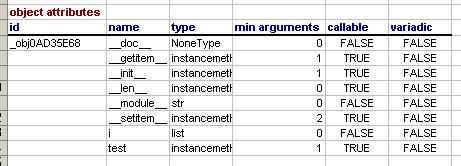
\includegraphics[width=11cm]{images/listallattr.jpg}
\end{xlpfunc}
\end{xlpfunctitle}

\subsection{xlpAttrInfos}

\begin{xlpfunctitle}{xlpAttrInfos}

\begin{xlpfunc}{Parameters}
\begin{tabular}{p{3.5cm}cl}
\textbf{scalar}& : & scalar code \\
\textbf{attr}& : & attribute name (character string) \\
\textbf{transpose}& : & transpose of output \\
\textbf{trigger}& : & trigger 
\end{tabular}
\end{xlpfunc}


\begin{xlpfunc}{Returns}
Cell matrix of dimension (4, 1).
\end{xlpfunc}

\begin{xlpfunc}{Description}
List all the attributes of the scalar code:
\begin{itemize}
\item the column 1 is the type
\item the column 2 is the minimum number of arguments
\item the column 3 say if the attribute is callable (a function)
\item the column 4 say if the attribute can accept a variable number of arguments (for function only).
\end{itemize}
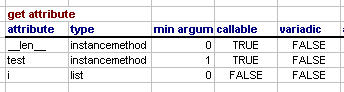
\includegraphics[width=11cm]{images/getattribute.jpg}
\end{xlpfunc}

\end{xlpfunctitle}

\section{Output functions}


\subsection{xlpIO}

\begin{xlpfunctitle}{xlpIO}

\begin{xlpfunc}{Parameters}
\begin{tabular}{p{3.5cm}cl}
\textbf{lines}& : & number of lines \\
\textbf{trigger}& : & trigger 
\end{tabular}
\end{xlpfunc}


\begin{xlpfunc}{Returns}
A cell matrix of dimension (lines, 3)
\end{xlpfunc}

\begin{xlpfunc}{Description}
\xlp has a circular buffer of 2048 lines storing the standart ouput messages coming from python or c++ (stdout, stderr, std::cout, std::cerr). This function allows to retrieve a view of the last messages. The argument lines give the number of messages that the function will show.


\

The first column represent the message index, the second column the origin of the message (stdout, stderr, std::cout, std::cerr), and the last column displays the message itself. 

\

The messages coming from python are identical to those that you can see on a python console ... could be very useful for debugging.

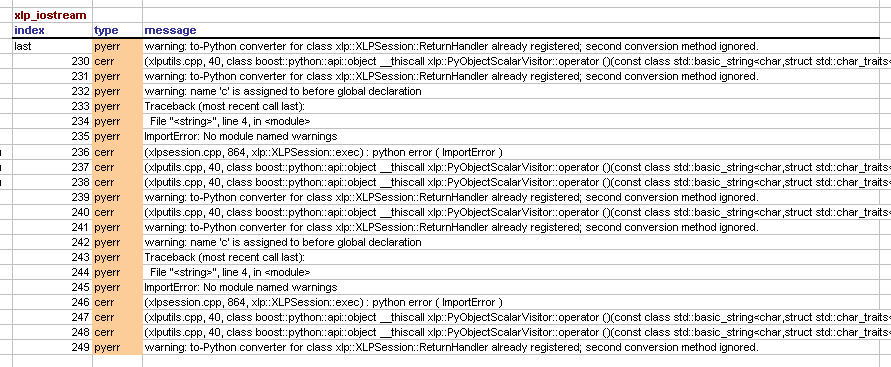
\includegraphics[width=14cm]{images/io.jpg}
\end{xlpfunc}
\end{xlpfunctitle}

\subsection{xlpFullIO}

\begin{xlpfunctitle}{xlpFullIO}

\begin{xlpfunc}{Parameters}
\begin{tabular}{p{3.5cm}cl}
\textbf{trigger}& : & trigger 
\end{tabular}
\end{xlpfunc}


\begin{xlpfunc}{Returns}
A cell matrix of dimension (2048, 3)
\end{xlpfunc}

\begin{xlpfunc}{Description}
\xlp has a circular buffer of 2048 lines storing the standart ouput messages coming from python or c++ (stdout, stderr, std::cout, std::cerr). This function allow to retrieve all the buffer. 

\

The first column represent the message index, the second column the origin of the message (stdout, stderr, std::cout, std::cerr), and the last column store the message itself. 
\end{xlpfunc}
\end{xlpfunctitle}



\section{Tool functions}


\subsection{xlpArgs}

\begin{xlpfunctitle}{xlpArgs}

\begin{xlpfunc}{Parameters}
\begin{tabular}{p{3.5cm}cl}
\textbf{args01}& : & cell list arguments 01 \\
\textbf{args02}& : & cell list arguments 02 \\
\textbf{args03}& : & cell list arguments 03 \\
\textbf{args04}& : & cell list arguments 04 \\
\textbf{args05}& : & cell list arguments 05 \\
\textbf{transpose}& : & transpose \\
\textbf{trigger}& : & trigger 
\end{tabular}
\end{xlpfunc}


\begin{xlpfunc}{Returns}
A cell matrix of dimension (n, 1) where n is the sum of the size of all list arguments.
\end{xlpfunc}

\begin{xlpfunc}{Description}
This function allows to concatenate various cell lists into one cell list.
This function is dedicated to be used in the call to other functions as {\it args} parameter.

Imagine that you have a volatiliy term structure depending on time and strike. Imagine that your object has an associated method called {\it blackVol} taking two parameters, time and strike. You want to fill a grid of volatilities like in the image below:

\

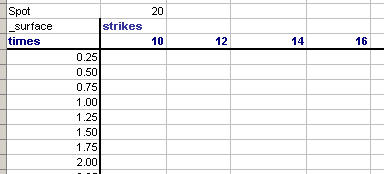
\includegraphics[width=11cm]{images/surface.jpg}

The function call in each cell will be similar to:

\begin{center}
{\sl xlpGetAttr($A$38,"blackVol",xlpArgs($A40,B$39, $B$37),,$C$21)}
\end{center}

\

Where you can see the usage of xlpArgs to create a cross reference args parameter from the times and the strikes. 

\

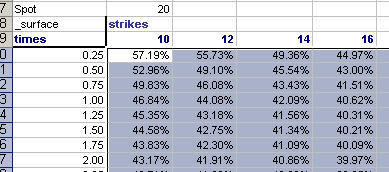
\includegraphics[width=11cm]{images/surface3.jpg}
\end{xlpfunc}
\end{xlpfunctitle}


\subsection{xlpBigArgs}

\begin{xlpfunctitle}{xlpBigArgs}

\begin{xlpfunc}{Parameters}
\begin{tabular}{p{3.5cm}cl}
\textbf{args01}& : & cell list arguments 01 \\
\textbf{args02}& : & cell list arguments 02 \\
\textbf{args03}& : & cell list arguments 03 \\
\textbf{args04}& : & cell list arguments 04 \\
\textbf{args05}& : & cell list arguments 05 \\
\textbf{args06}& : & cell list arguments 06 \\
\textbf{args07}& : & cell list arguments 07 \\
\textbf{args08}& : & cell list arguments 08 \\
\textbf{args09}& : & cell list arguments 09 \\
\textbf{args10}& : & cell list arguments 10 \\
\textbf{args11}& : & cell list arguments 11 \\
\textbf{args12}& : & cell list arguments 12 \\
\textbf{args13}& : & cell list arguments 13 \\
\textbf{args14}& : & cell list arguments 14 \\
\textbf{args15}& : & cell list arguments 15 \\
\textbf{args16}& : & cell list arguments 16 \\
\textbf{args17}& : & cell list arguments 17 \\
\textbf{args18}& : & cell list arguments 18 \\
\textbf{transpose}& : & transpose \\
\textbf{trigger}& : & trigger 
\end{tabular}
\end{xlpfunc}


\begin{xlpfunc}{Returns}
A cell matrix of dimension (n, 1) where n is the sum of the size of all list arguments.
\end{xlpfunc}

\begin{xlpfunc}{Description}
Like xlpArgs.
\end{xlpfunc}
\end{xlpfunctitle}


\subsection{xlpTranspose}

\begin{xlpfunctitle}{xlpTranspose}

\begin{xlpfunc}{Parameters}
\begin{tabular}{p{3.5cm}cl}
\textbf{scalars}& : & cell matrix \\
\textbf{trigger}& : & trigger 
\end{tabular}
\end{xlpfunc}


\begin{xlpfunc}{Returns}
A cell matrix of dimension (m, n) where n is the number of rows and m the number of columns of the imput cell matrix.
\end{xlpfunc}

\begin{xlpfunc}{Description}
Transpose a cell matrix.
\end{xlpfunc}
\end{xlpfunctitle}




\subsection{xlpTrigger}

\begin{xlpfunctitle}{xlpTrigger}

\begin{xlpfunc}{Parameters}
\begin{tabular}{p{3.5cm}cl}
\textbf{trigger01}& : & trigger 01 \\
\textbf{trigger02}& : & trigger 02 \\
\textbf{trigger03}& : & trigger 03 \\
\textbf{trigger04}& : & trigger 04 \\
\textbf{trigger05}& : & trigger 05 \\
\end{tabular}
\end{xlpfunc}


\begin{xlpfunc}{Returns}
An index.
\end{xlpfunc}

\begin{xlpfunc}{Description}
Return FALSE if one of the trigger is in error or FALSE. Otherwise it return an incressing index.
\end{xlpfunc}
\end{xlpfunctitle}

\subsection{xlpBigTrigger}

\begin{xlpfunctitle}{xlpBigTrigger}

\begin{xlpfunc}{Parameters}
\begin{tabular}{p{3.5cm}cl}
\textbf{trigger01}& : & trigger 01 \\
\textbf{trigger02}& : & trigger 02 \\
\textbf{trigger03}& : & trigger 03 \\
\textbf{trigger04}& : & trigger 04 \\
\textbf{trigger05}& : & trigger 05 \\
\textbf{trigger06}& : & trigger 06 \\
\textbf{trigger07}& : & trigger 07 \\
\textbf{trigger08}& : & trigger 08 \\
\textbf{trigger09}& : & trigger 09 \\
\textbf{trigger10}& : & trigger 10 \\
\textbf{trigger11}& : & trigger 11 \\
\textbf{trigger12}& : & trigger 12 \\
\textbf{trigger13}& : & trigger 13 \\
\textbf{trigger14}& : & trigger 14 \\
\textbf{trigger15}& : & trigger 15 \\
\textbf{trigger16}& : & trigger 16 \\
\textbf{trigger17}& : & trigger 17 \\
\textbf{trigger18}& : & trigger 18 \\
\textbf{trigger19}& : & trigger 19 \\
\textbf{trigger20}& : & trigger 20 \\
\end{tabular}
\end{xlpfunc}


\begin{xlpfunc}{Returns}
An index.
\end{xlpfunc}

\begin{xlpfunc}{Description}
Return FALSE if one of the trigger is in error or FALSE. Otherwise it return an incressing index.
\end{xlpfunc}
\end{xlpfunctitle}


\subsection{xlpTranspose}

\begin{xlpfunctitle}{xlpTranspose}

\begin{xlpfunc}{Parameters}
\begin{tabular}{p{3.5cm}cl}
\textbf{scalars}& : & cell matrix \\
\textbf{trigger}& : & trigger 
\end{tabular}
\end{xlpfunc}


\begin{xlpfunc}{Returns}
A cell matrix of dimension (m, n) where n is the number of rows and m the number of columns of the imput cell matrix.
\end{xlpfunc}

\begin{xlpfunc}{Description}
Transpose a cell matrix.
\end{xlpfunc}
\end{xlpfunctitle}




\subsection{xlpAdjustShape}

\begin{xlpfunctitle}{xlpAdjustShape}

\begin{xlpfunc}{Parameters}
\begin{tabular}{p{3.5cm}cl}
\textbf{scalars}& : & cell matrix \\
\textbf{rows}& : & number of rows \\
\textbf{columns}& : & number of columns \\
\textbf{trigger}& : & trigger 
\end{tabular}
\end{xlpfunc}


\begin{xlpfunc}{Returns}
A cell matrix of dimension (rows, columns) where $rows * columnns$ is  equal to $rows\_input\_matrix * columns\_input\_matrix$.  
\end{xlpfunc}

\begin{xlpfunc}{Description}
Transpose a cell matrix.
\end{xlpfunc}
\end{xlpfunctitle}


\subsection{xlpLoadFile}

\begin{xlpfunctitle}{xlpLoadFile}

\begin{xlpfunc}{Parameters}
\begin{tabular}{p{3.5cm}cl}
\textbf{file}& : & filename \\
\textbf{id}& : & object id \\
\textbf{trigger}& : & trigger 
\end{tabular}
\end{xlpfunc}


\begin{xlpfunc}{Returns}
A character string representing the object id
\end{xlpfunc}

\begin{xlpfunc}{Description}
Load a file referenced by filename and store it as a character string python object. 
\end{xlpfunc}
\end{xlpfunctitle}


\subsection{xlpVolatile}

\begin{xlpfunctitle}{xlpVolatile}

\begin{xlpfunc}{Parameters}
\begin{tabular}{p{3.5cm}cl}
\textbf{trigger}& : & trigger 
\end{tabular}
\end{xlpfunc}


\begin{xlpfunc}{Returns}
A real number.
\end{xlpfunc}

\begin{xlpfunc}{Description}
The function return a incremental number. This function is volatile, that mean that Excel calls it every time that a change occureds on the sheet.
\end{xlpfunc}
\end{xlpfunctitle}

\subsection{xlpReduce}

\begin{xlpfunctitle}{xlpReduce}

\begin{xlpfunc}{Parameters}
\begin{tabular}{p{3.5cm}cl}
\textbf{args}& : & arguments \\
\textbf{transpose}& : & output transpose \\
\textbf{trigger}& : & trigger 
\end{tabular}
\end{xlpfunc}


\begin{xlpfunc}{Returns}
A cell matrix.
\end{xlpfunc}

\begin{xlpfunc}{Description}
The function reduce a cell matrix into another matrix eliminating the error or missing cell. This function can handle only matrix where there is full rows or full columns in error.
\end{xlpfunc}
\end{xlpfunctitle}


\subsection{xlpR}

\begin{xlpfunctitle}{xlpR}

\begin{xlpfunc}{Parameters}
\begin{tabular}{p{3.5cm}cl}
\textbf{args}& : & arguments \\
\textbf{transpose}& : & output transpose \\
\textbf{trigger}& : & trigger 
\end{tabular}
\end{xlpfunc}


\begin{xlpfunc}{Returns}
A cell matrix.
\end{xlpfunc}

\begin{xlpfunc}{Description}
Shortcut for xlpReduce.
\end{xlpfunc}
\end{xlpfunctitle}


\subsection{xlpPretty}

\begin{xlpfunctitle}{xlpPretty}

\begin{xlpfunc}{Parameters}
\begin{tabular}{p{3.5cm}cl}
\textbf{args}& : & arguments \\
\textbf{transpose}& : & output transpose \\
\textbf{trigger}& : & trigger 
\end{tabular}
\end{xlpfunc}


\begin{xlpfunc}{Returns}
A cell matrix.
\end{xlpfunc}

\begin{xlpfunc}{Description}
Get a pretty matrix. This function cannot be called inside another \xlp function.
Try it for explanation.
\end{xlpfunc}
\end{xlpfunctitle}


\subsection{xlpP}

\begin{xlpfunctitle}{xlpP}

\begin{xlpfunc}{Parameters}
\begin{tabular}{p{3.5cm}cl}
\textbf{args}& : & arguments \\
\textbf{transpose}& : & output transpose \\
\textbf{trigger}& : & trigger 
\end{tabular}
\end{xlpfunc}


\begin{xlpfunc}{Returns}
A cell matrix.
\end{xlpfunc}

\begin{xlpfunc}{Description}
Shortcut for xlpPretty.
\end{xlpfunc}
\end{xlpfunctitle}

\subsection{xlpTime}

\begin{xlpfunctitle}{xlpTime}

\begin{xlpfunc}{Parameters}
\begin{tabular}{p{3.5cm}cl}
\textbf{trigger}& : & trigger 
\end{tabular}
\end{xlpfunc}


\begin{xlpfunc}{Returns}
A real number.
\end{xlpfunc}

\begin{xlpfunc}{Description}
Return a real number representing the time in second since the add-in has been loaded. 
The aim of this function is to allow calculating execution time of a function.
\end{xlpfunc}
\end{xlpfunctitle}



\section{Inbformation functions}

\subsection{xlpVersion}

\begin{xlpfunctitle}{xlpVersion}
\begin{xlpfunc}{Parameters}
\begin{tabular}{p{3.5cm}cl}
\textbf{trigger}& : & trigger \\
\end{tabular}
\end{xlpfunc}


\begin{xlpfunc}{Returns}
A cell matrix of dimension (1, 1)
\end{xlpfunc}

\begin{xlpfunc}{Description}
Return the \xlp version.
\end{xlpfunc}
\end{xlpfunctitle}


\subsection{xlpAuthor}

\begin{xlpfunctitle}{xlpAuthor}
\begin{xlpfunc}{Parameters}
\begin{tabular}{p{3.5cm}cl}
\textbf{trigger}& : & trigger \\
\end{tabular}
\end{xlpfunc}


\begin{xlpfunc}{Returns}
A cell matrix of dimension (1, 1)
\end{xlpfunc}

\begin{xlpfunc}{Description}
Return the \xlp author.
\end{xlpfunc}
\end{xlpfunctitle}

\subsection{xlpContributors}


\begin{xlpfunctitle}{xlpContributors}
\begin{xlpfunc}{Parameters}
\begin{tabular}{p{3.5cm}cl}
\textbf{trigger}& : & trigger \\
\end{tabular}
\end{xlpfunc}


\begin{xlpfunc}{Returns}
A cell matrix of dimension (n, 1)
\end{xlpfunc}

\begin{xlpfunc}{Description}
Return the \xlp contributors.
\end{xlpfunc}
\end{xlpfunctitle}


\subsection{xlpPythonPath}

\begin{xlpfunctitle}{xlpPythonPath}
\begin{xlpfunc}{Parameters}
\begin{tabular}{p{3.5cm}cl}
\textbf{trigger}& : & trigger \\
\end{tabular}
\end{xlpfunc}


\begin{xlpfunc}{Returns}
A cell matrix of dimension (1, 1)
\end{xlpfunc}

\begin{xlpfunc}{Description}
Return the PYTHONPATH environment variable.
\end{xlpfunc}
\end{xlpfunctitle}



\subsection{xlpPythonVersion}

\begin{xlpfunctitle}{xlpPythonVersion}
\begin{xlpfunc}{Parameters}
\begin{tabular}{p{3.5cm}cl}
\textbf{trigger}& : & trigger \\
\end{tabular}
\end{xlpfunc}


\begin{xlpfunc}{Returns}
A cell matrix of dimension (1, 1)
\end{xlpfunc}

\begin{xlpfunc}{Description}
Return the python version.
\end{xlpfunc}
\end{xlpfunctitle}


\subsection{xlpSysPath}

\begin{xlpfunctitle}{xlpSysPath}
\begin{xlpfunc}{Parameters}
\begin{tabular}{p{3.5cm}cl}
\textbf{trigger}& : & trigger \\
\end{tabular}
\end{xlpfunc}


\begin{xlpfunc}{Returns}
A cell matrix of dimension (1, n)
\end{xlpfunc}

\begin{xlpfunc}{Description}
Return the system paths.
\end{xlpfunc}
\end{xlpfunctitle}
%\include{concept}

\chapter{Tutorial 1: creating a Matrix class available in Excel}


As I have mentioned before, \xlp has a generic way to handle container. In this tutorial we will look at this method and will create a matrix class than can be directly handled by \xlp. 


\section{A class Matrix}


Below the definition of a Matrix class compatible with \xlp.

\

\begin{verbatim}
class Matrix:
 
	def __init__(self, rows, cols):
 		self.rows = rows
 		self.cols = cols
  	self.datas = range(self.rows*self.cols)

 	def __len__(self): 
  	return len(self.datas)

 	def __setitem__(self, index, value):
  	self.datas.__setitem__(index, value)

 	def __getitem__(self, index):
  	return self.datas.__getitem__(index)
 
 	def size1(self):
  	return self.rows
  	
  def size2(self):
  	return self.cols
  	
\end{verbatim}

\

You can see that we need to define the methods \_\_len\_\_, \_\_setitem\_\_,  \_\_getitem\_\_, size1 and size2.

\

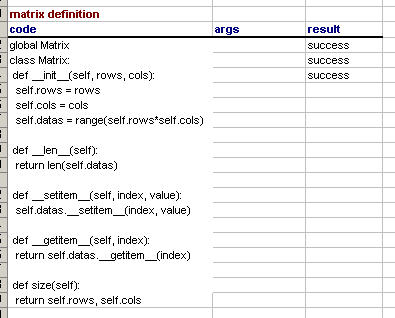
\includegraphics[width=12cm]{images/matrix1.jpg}


\section{Matrix creation}

To create the matrix, we need to generate an empty matrix with correct dimensions "\_Matrix(\_rows, \_cols)" and fill it with the values arguments. 

\ 

Here the result:

\

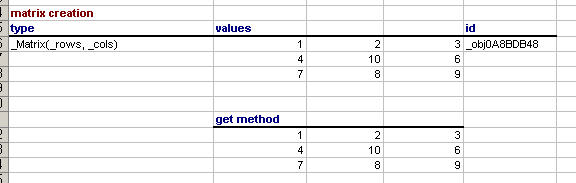
\includegraphics[width=12cm]{images/matrix2.jpg}


\chapter{Tutorial 2: computing time calculation}


In that tutorial we will see how to calculate the time computation of a script in \xlp with the use of the trigger parameter and xlpTime function.

\section{A script}

Here the script that we will test:

\

for x in range(0,\_1):

 print x
 
 
\section{Linking functions with the trigger parameter}

In order to compute the time, we need to make a call to xlpTime twice:
\begin{itemize}
\item one before the call to the script
\item one after the execution of the script.
\end{itemize}

\

In order to allow synchronisation we will make the first call to xlpTime will be linked to a cell trigger by the use of the parameter trigger. The execution of the script wil be linked to the result of the first call at xlpTime via the trigger parameter. Finally the last call to xlpTime will be linked to the result of the script.

\

Here the result:

\

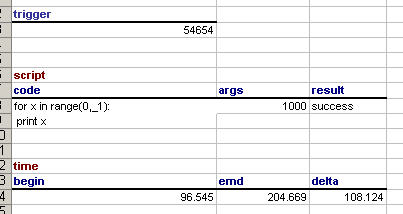
\includegraphics[width=12cm]{images/timecomp.jpg}

\



\chapter{Tutorial 3: Extraction data from Front Arena to Excel - Correlation Extraction}

Extraction of data from Front Arena to Excel is now directly possible. 


\section{Fron Arena connection session}

Before getting data, we need to connect to Front Arena. As Front Arena does not accept multiple connection of the same user we need to create a singleton class. That is the aim of the class FrontArenaSession:

\begin{verbatim}

class FrontArenaSession:
    
    class __Impl:
        
        def __init__(self, server, userid, password):
            import sys
            sys.path.insert(0, r'C:\Program Files\Front\Front Arena42\Prime\4.2')
            self.ael = __import__('ael')
            self.acm = __import__('acm')
            self.ael.connect(server, userid, password)
 
        def __del__(self):
            self.ael.disconnect()
            
        def today(self):
            return self.ael.date_today()
        
        def excel_date(self, ael_date):
            return self.ael.date_from_string('1899-12-30').days_between(ael_date)
        
        def ael_date(self, excel_date):
            return self.ael.date_from_string('1899-12-30').add_days(excel_date)
                        
    __instance = {}
 
    def __init__(self, server, userid, password):
        self._key = (server, userid, password)
        if not FrontArenaSession.__instance.has_key(self._key):
            FrontArenaSession.__instance[self._key] = FrontArenaSession.__Impl(server, userid, password)
    
    def __getattr__(self, name):
        if not name == '_key':
            return getattr(self.__instance[self._key], name)
 
    def __setattr__(self, aAttr, aValue):
        if not aAttr == '_key':
            return setattr(self.__instance[self._key], aAttr, aValue)
            
\end{verbatim} 

\section{A data manager class}

\begin{verbatim}
class DataManager:

    def __init__(self, session):
        self._session = session

    def getCorrelation(self, name):
        corr = self._session.ael.CorrelationMatrix[name].correlations()
        index={}
        pairs={}
        for member in corr:   
            first = self._session.ael.Instrument[member.recaddr0].insid
            second = self._session.ael.Instrument[member.recaddr1].insid
            pairs[(first,second)] = member.corr    
            index[first] = None
            index[second] = None
        index = index.keys()
        index.sort()
        return CorrelationMatrix(index, pairs, name)
\end{verbatim}


\section{A correlation class}

\begin{verbatim}
class Matrix:

    def __init__(self, rows, cols):
        self._rows = rows
        self._cols = cols
        self._datas = range(0, rows*cols)

    def __getitem__(self, index):
        return self._datas.__getitem__(index)

    def __setitem__(self, index, value):
        self._datas.__setitem__(index, value)

    def __len__(self):
        return len(self._datas)

    def size1(self):
        return self._rows
        
    def size2(self):
        return self._cols

    def operator(x, y):
        if (x > self._rows) or (y > self._cols) or (x < 0) or (y < 0):
            raise Exception , "bad value for index"
        return self._datas[x*self._cols+y]


class CorrelationMatrix:

    def __init__(self, instruments, corrPairs, name):
        self.instruments = instruments
        self._corrPairs = corrPairs
        self.matrix = Matrix(len(instruments), len(instruments))
        self.name = name
        for x in instruments:
            self._corrPairs[(x, x)] = 1.0
        offset = 0
        for x in instruments:
            for y in instruments:
                val = 0.0
                try:
                    val = self._corrPairs[(x, y)] 
                except:
                    val = self._corrPairs[(y, x)]
                self.matrix.__setitem__(offset, val) 
                offset += 1
        
    def correlation(self, inst1, inst2):
        try:
            return self._corrPairs[(inst1, inst2)]
        except:
            return self._corrPairs[(inst2, inst1)]
          
\end{verbatim}

\section{Putting all together} 

Go to see the file correlationtutorial.xls to see the result.

\chapter{Tutorial 4: using Front Arena AEL and ACM librairies in Excel}

Go to see the file dataextraction-tutorial.xll and FrontArena.py. Verify that your PYTHONPATH is defined and that FrontArena.py it is accessible.


\appendix

%\listoftables
\listoffigures

%\addcontentsline{toc}{chapter}{Bibliographie}
%\bibliography{biblio}
\end{document}
